\chapter{Troubleshoot the \zwave Network}
\label{c5:cit}

The \zweui is perfectly suited to troubleshoot networks and find and 
fix problems.  Troubleshooting a \zwave network works along the lines of the communication stack.

Problems can occur on the radio layer, the networking layer, and the application layer. To 
identify and fix problems, it makes sense to work bottom up through the network stack issues.

Most of the troubleshooting functions are accessible on the menu item \menu{Analytics.} However, 
this menu item will only be displayed if the firmware on the \zwave chip supports some special 
functions needed for troubleshooting purpose.

\section{Radio Layer}

\begin{figure}
\begin{center}
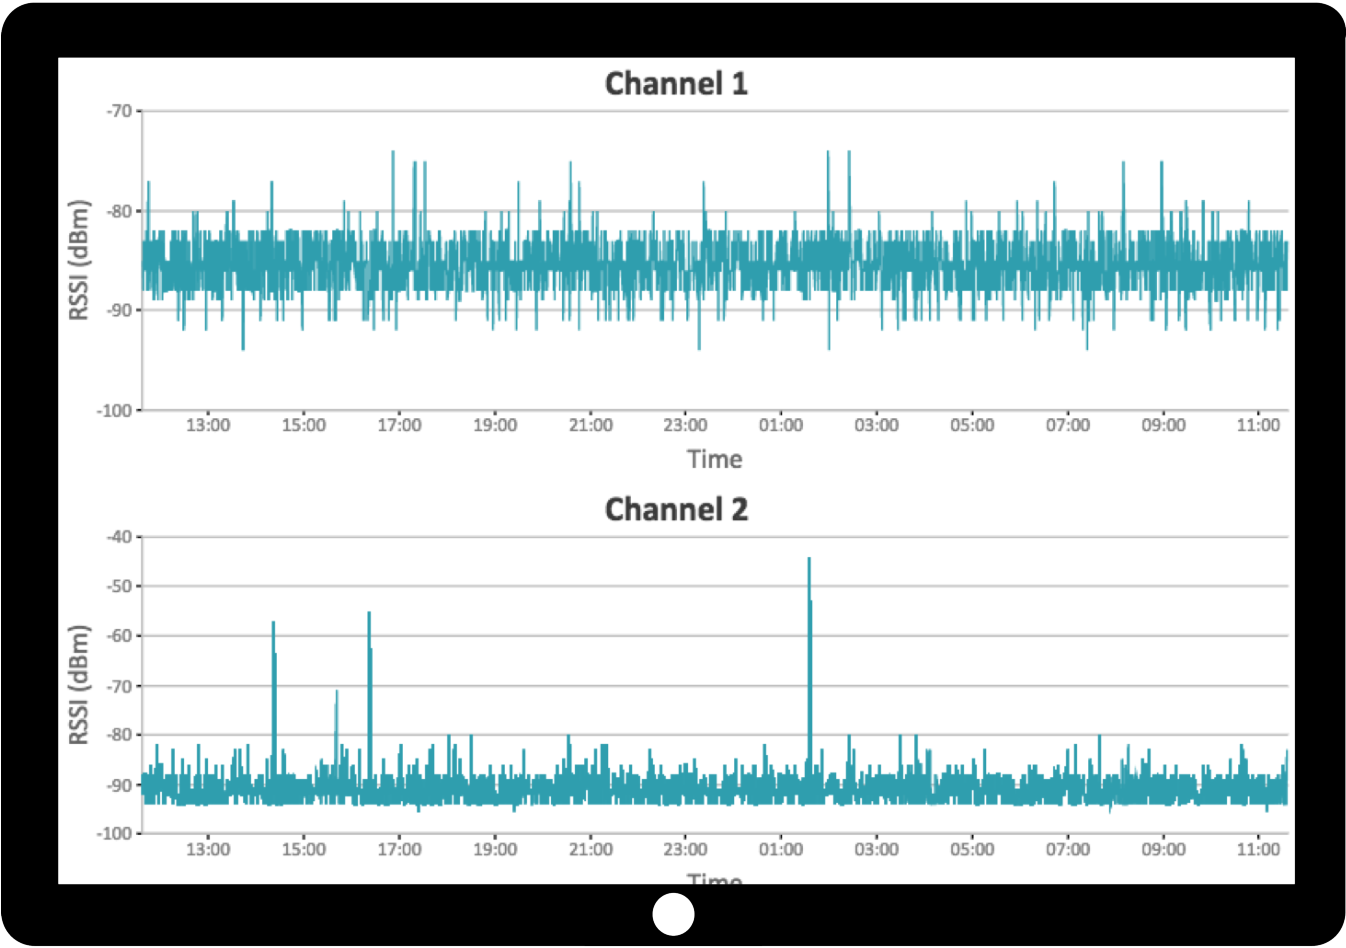
\includegraphics[width=0.7\textwidth]{pngs/cap8/c2backgroundnoise.pdf}
\caption{Background Noise}
\label{c5:backgroundNoise}
\end{center}
\end{figure}

Problems on the radio layer come from interference and noise generated by defect or 
nonconforming electrical gear causing electromagnetic emissions (baby monitor, old cordless 
phones, wireless speakers, motors, etc.). Other \zwave networks with unusual high traffic 
can also be a root cause of problems. It is also possible that certain other wireless 
networking services (first and foremost cellular network G4 routers or base stations, also 
called LTE) may cause interference if they are too closed to the \zwave network.

The menu item \menu{Analytics > Background Noise} offers a view chart displaying the background 
noise on the two communication channels used by \zwave. Channel 1 refers to the 9.6 Kbit/s 
and 40 kbit/s communication modes, channel 2 points to the 100kbit/s data rate.
Figure \ref{c5:backgroundNoise} shows this viewgraph. There is an obvious floor of 
noise with some other ``needles.'' This noise floor---in Figure \ref{c5:backgroundNoise} 
at about -85 dBm for channel 1 and -90 dBm for channel 2---is the minimum level a \zwave 
transceivers signal must surpass in order to be decoded by the \zwave receiver.

\textbf{The lower the noise level the better the wireless situation.
Noise levels below - 95 dBm are very good, levels above -70 dBm are very bad.}

Please note that this noise level is measured right on the controllers location or wherever 
the hardware running \zway is positioned. It may make sense to move the measuring device around to see the 
noise level at different locations. Since the \menu{ Analytics > Background Noise} viewgraph is 
only updated once per minute, you may want to use the tool \menu{Analytics > Noise Gauge}, as 
shown in Figure \ref{c5:noisegauge}. In this case, the display is updated every two seconds.

\begin{figure}
\begin{center}
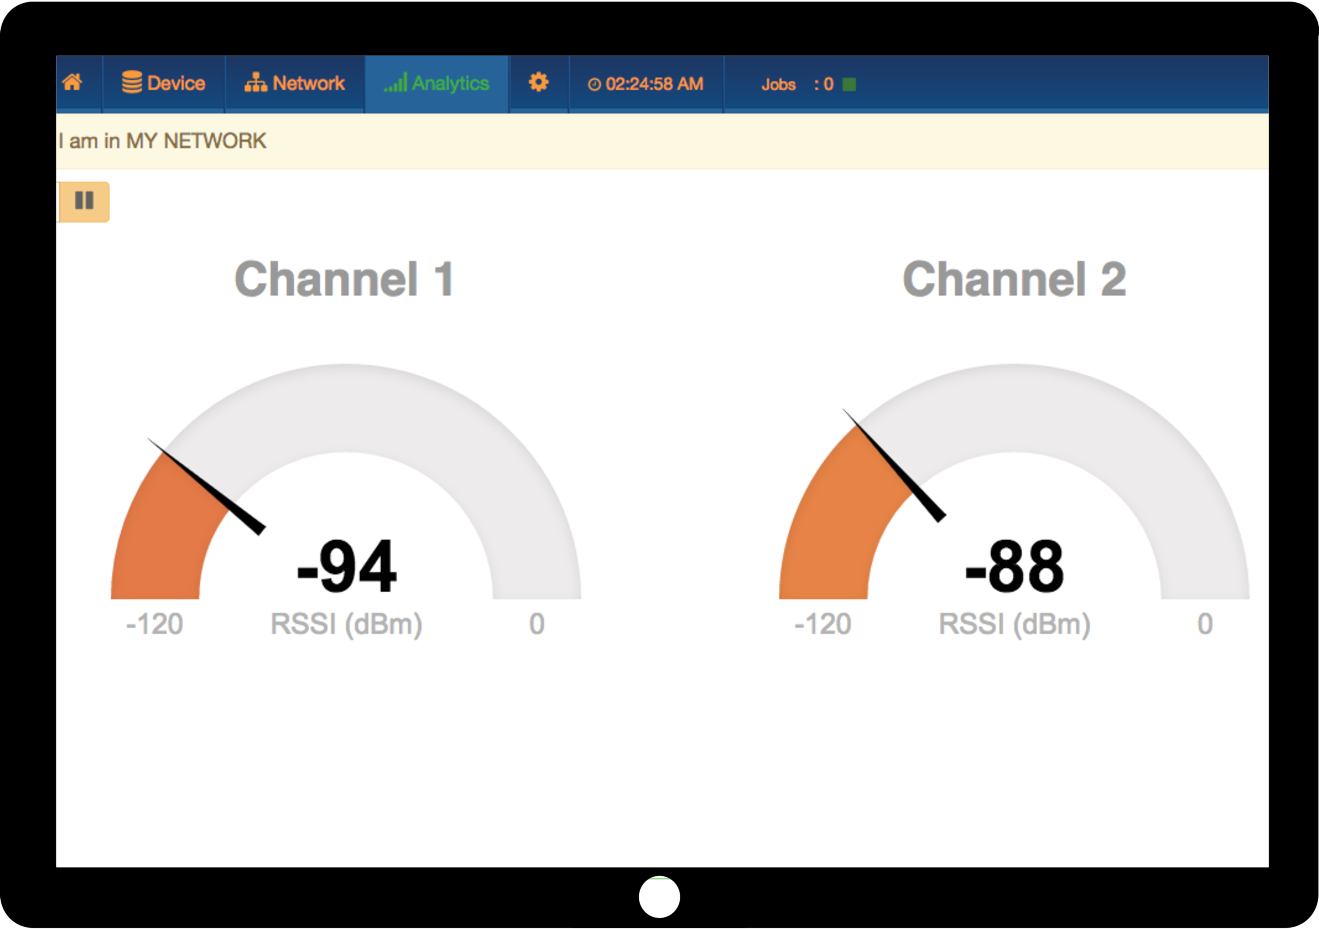
\includegraphics[width=0.7\textwidth]{pngs/cap8/c5noisegauge.pdf}
\caption{Realtime Measurement of Background-Noise}
\label{c5:noisegauge}
\end{center}
\end{figure}

\begin{figure}
\begin{center}
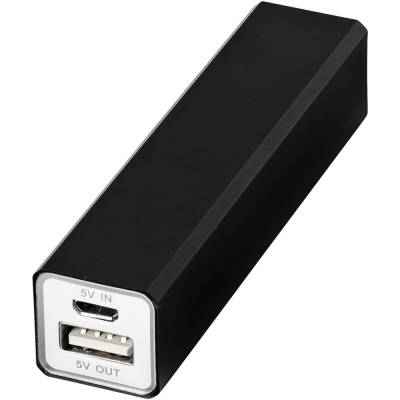
\includegraphics[width=0.4\textwidth]{pngs/cap8/powerbank.jpg}
\caption{Powerbank to power the \zway controller for mobile use}
\label{c5:powerbank}
\end{center}
\end{figure}

If the noise floor is too high, you need to find the source of the noise. The device running \zway can be 
used as mobile device too, thanks to the built-in Wi-Fi. In this case, it needs to be 
powered with a power bank as shown in Figure \ref{c5:powerbank}.

Walking around with the Noise Gauge enabled may help to track down the jamming device. The 
closer the controller hardware gets to the source of the noise, the higher the background noise level will be.

The ``needles'' above the noise floor show communication from other \zwave networks around. 
Having this is not a real problem unless other networks generate heavy traffic. A rule of 
thumb is that there should not be more than 30 \% of the time allocated by traffic of 
other \zwave networks. If there is more traffic, there will be a need to troubleshoot 
the other \zwave network first. The chart \menu{Analytics  > Network Statistics}, as shown 
in Figure \ref{c5:networkstat}, shows a ratio of own traffic versus traffic 
seen from other networks.

\begin{figure}
\begin{center}
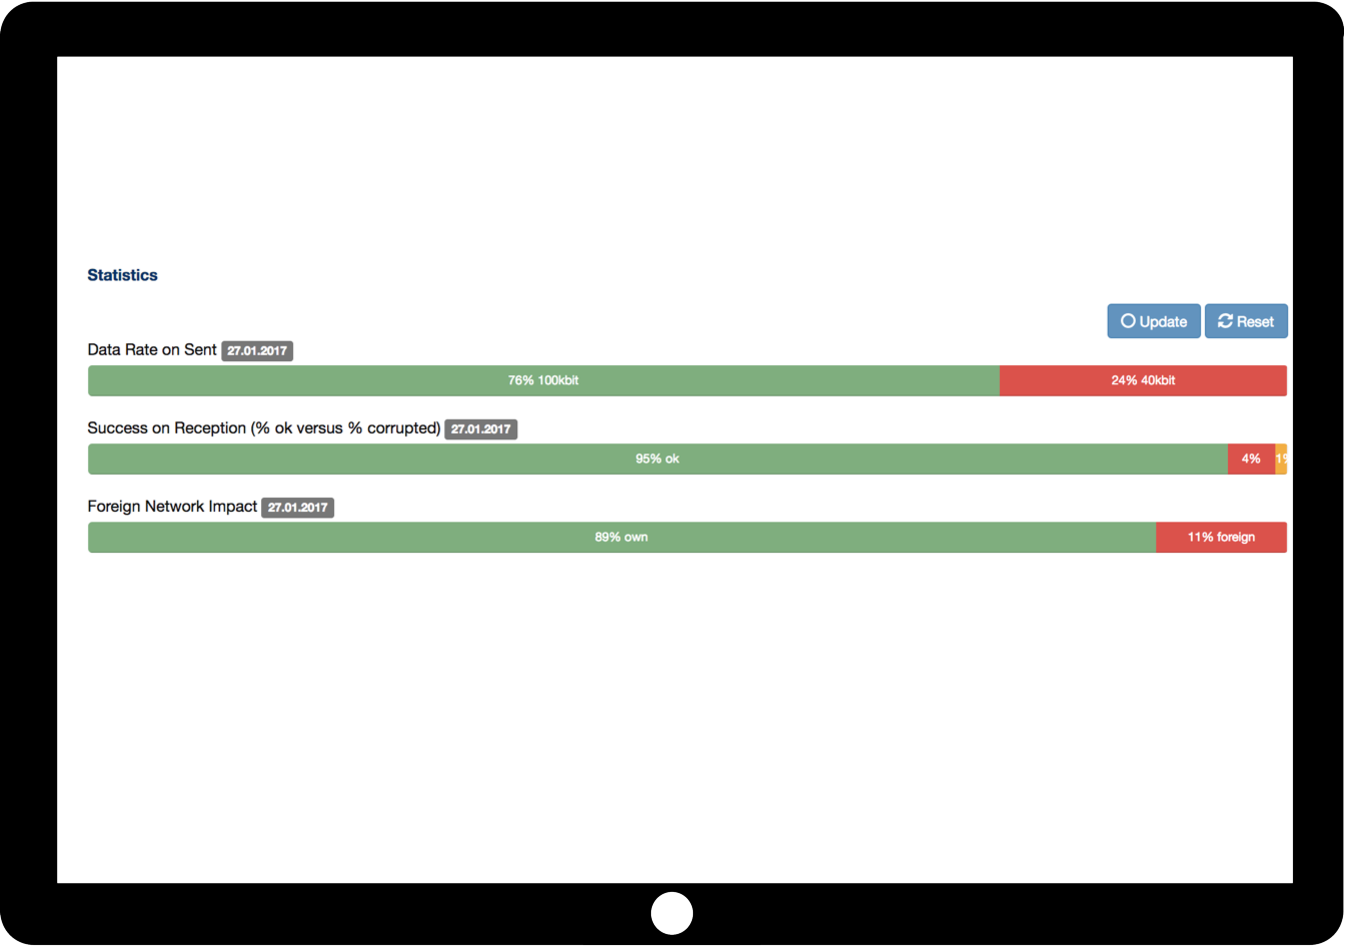
\includegraphics[width=0.7\textwidth]{pngs/cap8/c5networkstatistics.pdf}
\caption{Network Statistics Display}
\label{c5:networkstat}
\end{center}
\end{figure}

\section{Network Layer - Devices}

Devices can have two faulty states:

\begin{itemize}
\item They are dead, removed, faulty, stolen, etc. In case of a mains-operated device, 
the central \zway controller  will eventually find out that the device is not responding. 
It will put the device in the failed node list (for more information about failed node 
please refer to Chapter \ref{eui}). The \menu{ Devices  > Status Overview} as shown in 
Figure \ref{c5:citstatus} indicates if a device is failed or not.
It is possible to make a test if the device is working.
\item The device is working but constantly sending unsolicited messages. This is a rare 
but not impossible behavior. The simplest way to find out is to consider the packet 
sniffer. Figure \ref{c5:snifferpak} shows the \menu{Analytis > Sniffer View} of the \zweui.
\end{itemize}

\begin{figure}
\begin{center}
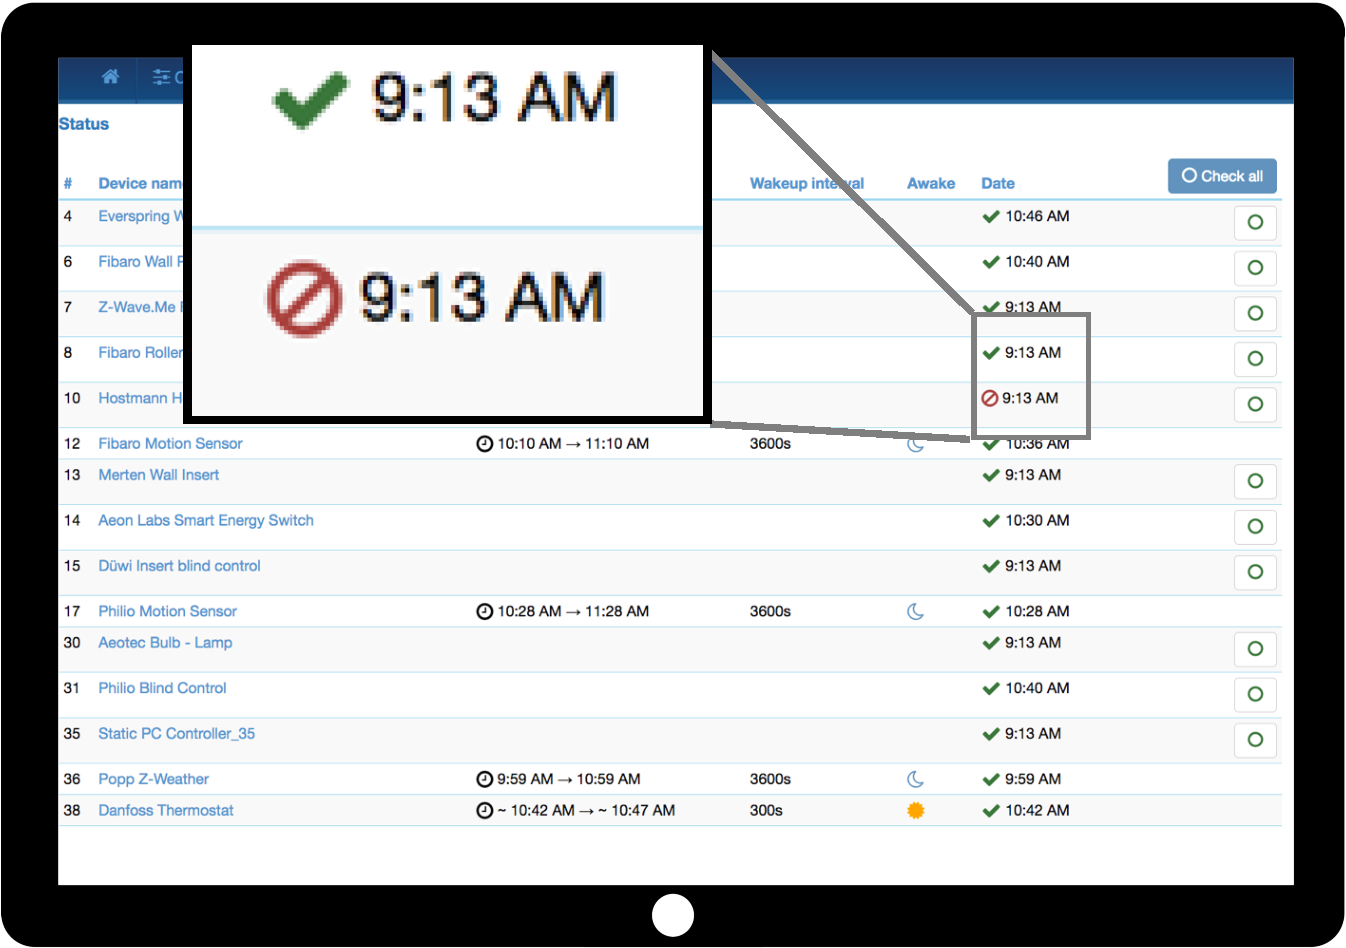
\includegraphics[width=0.7\textwidth]{pngs/cap8/c5networkstatus.pdf}
\caption{Status Page \zway}

\label{c5:citstatus}
\end{center}
\end{figure}


\begin{figure}
\begin{center}
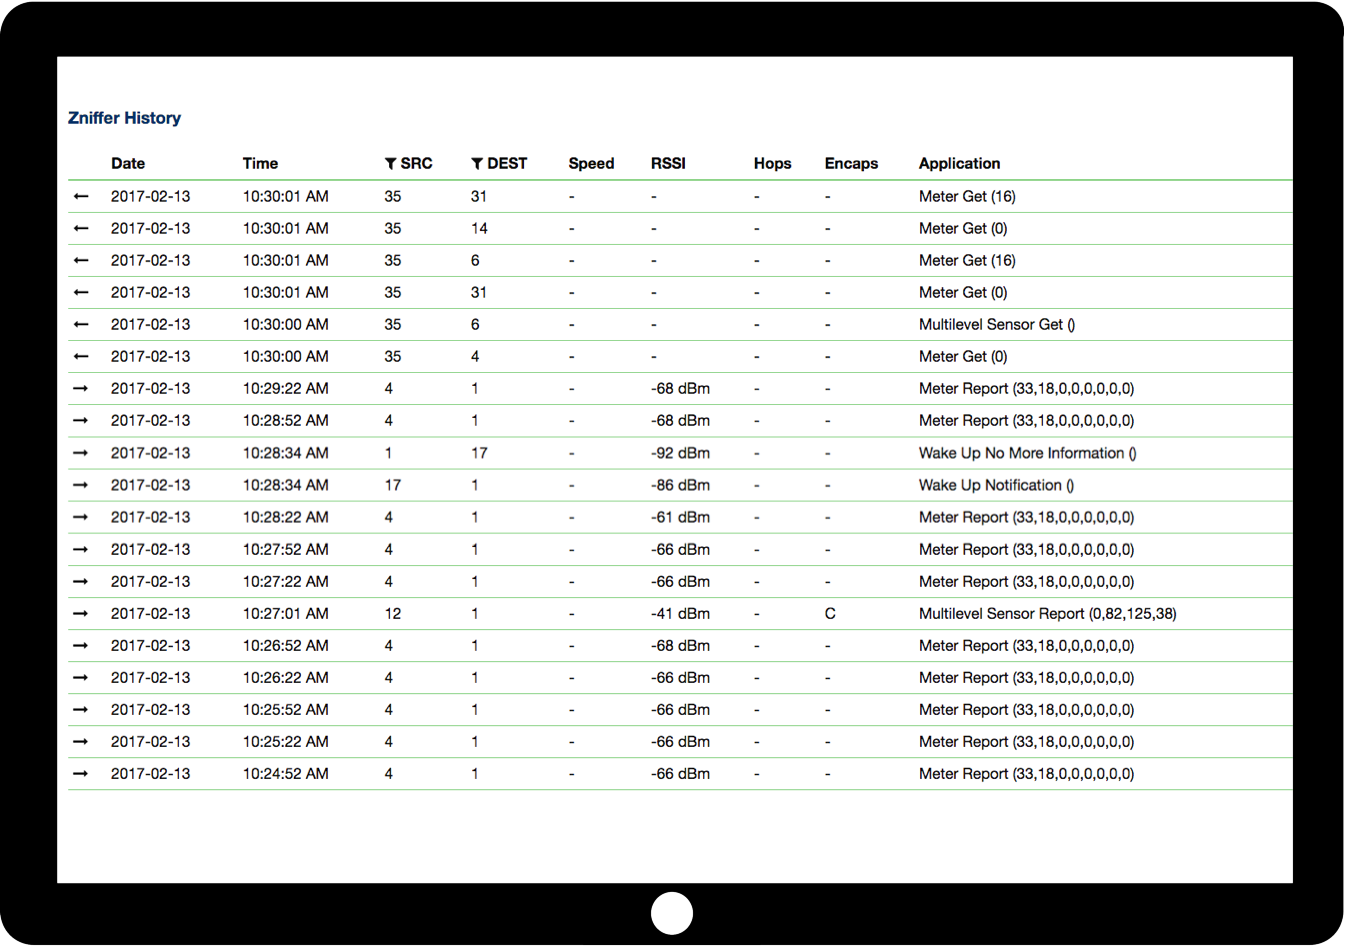
\includegraphics[width=0.7\textwidth]{pngs/cap8/c5sniffer.pdf}
\caption{Packet Sniffer}
\label{c5:snifferpak}
\end{center}
\end{figure}

Another option to detect faulty devices is the \menu{Network > Timing Info View}. 

\begin{figure}
\begin{center}
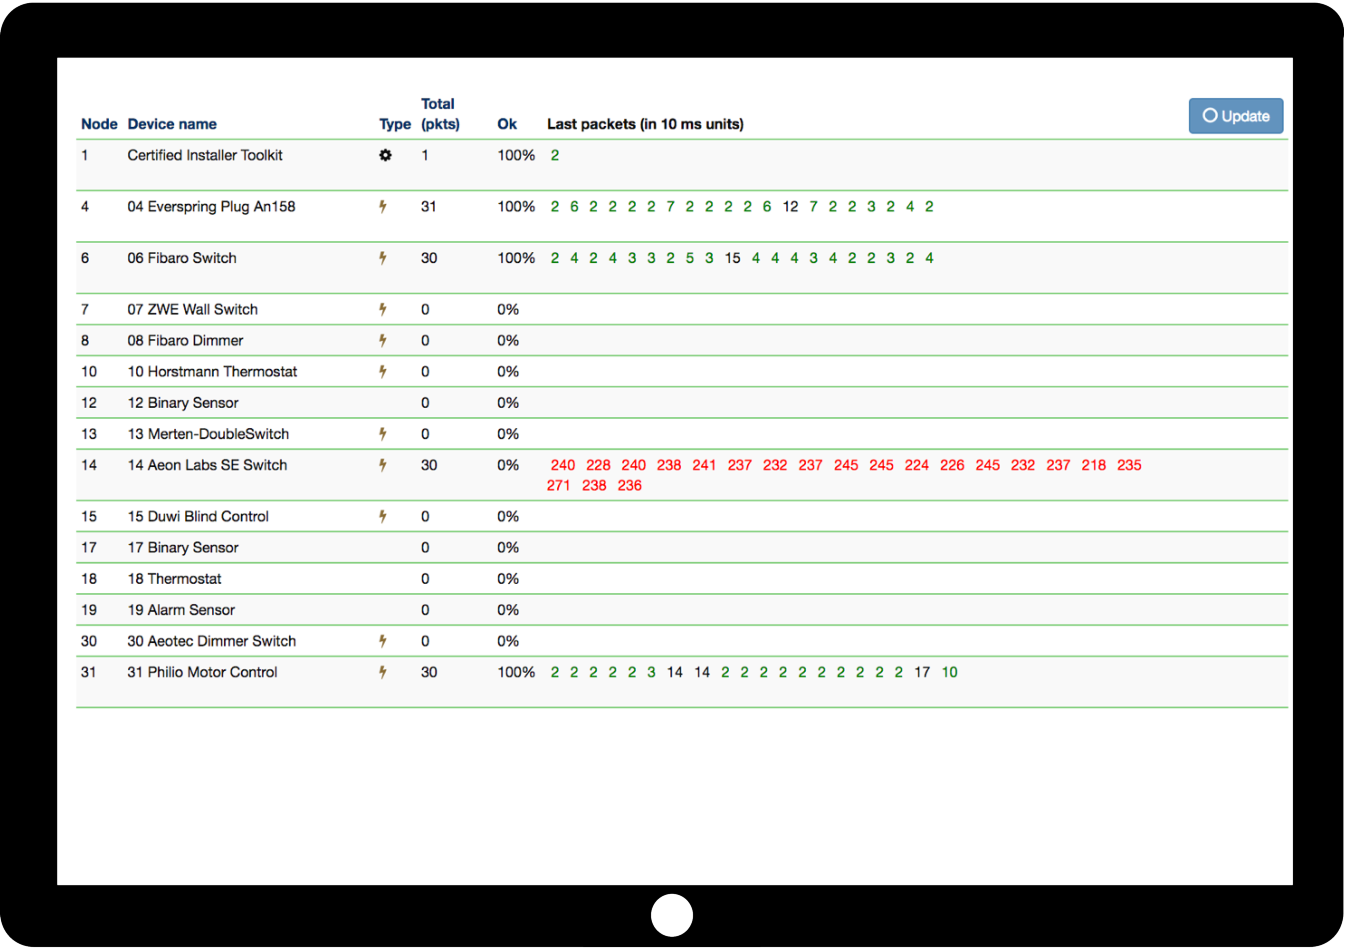
\includegraphics[width=0.7\textwidth]{pngs/cap8/c5timinginfo1.pdf}
\caption{Paket timing of a fresh \zwave network}
\label{c5:snifferfresh}
\end{center}
\end{figure}

Figure \ref{c5:snifferfresh} shows this view. The timing information lists one entry for 
every communication between the controller and the device. The number refers to the time 
(in x * 10 ms) the message took before being confirmed; the color gives a rough 
indication of what happened:

\begin{itemize}
\item Green: Successful communication with device in direct wireless range.
\item Black: Successful communication with device using a route.
\item Red: Failed communication (after a total of nine attempts).
\end{itemize}

Figure \ref{c5:snifferfresh} shows the situation in a network just installed. It can be 
seen that there is only communication with few devices, e.g. no polling of sensors, etc. 
While this is not a problem, the chart shows that devices 4, 6, and 31 are in direct 
range and all communication works perfectly well (green, low number). Device 14 seems 
to be a real problem child. The controller tries all the time to reach this node but 
always fails. At some point in time, the controller will accept that node 31 is dead 
and put him into the ``failed node list.''

\begin{figure}
\begin{center}
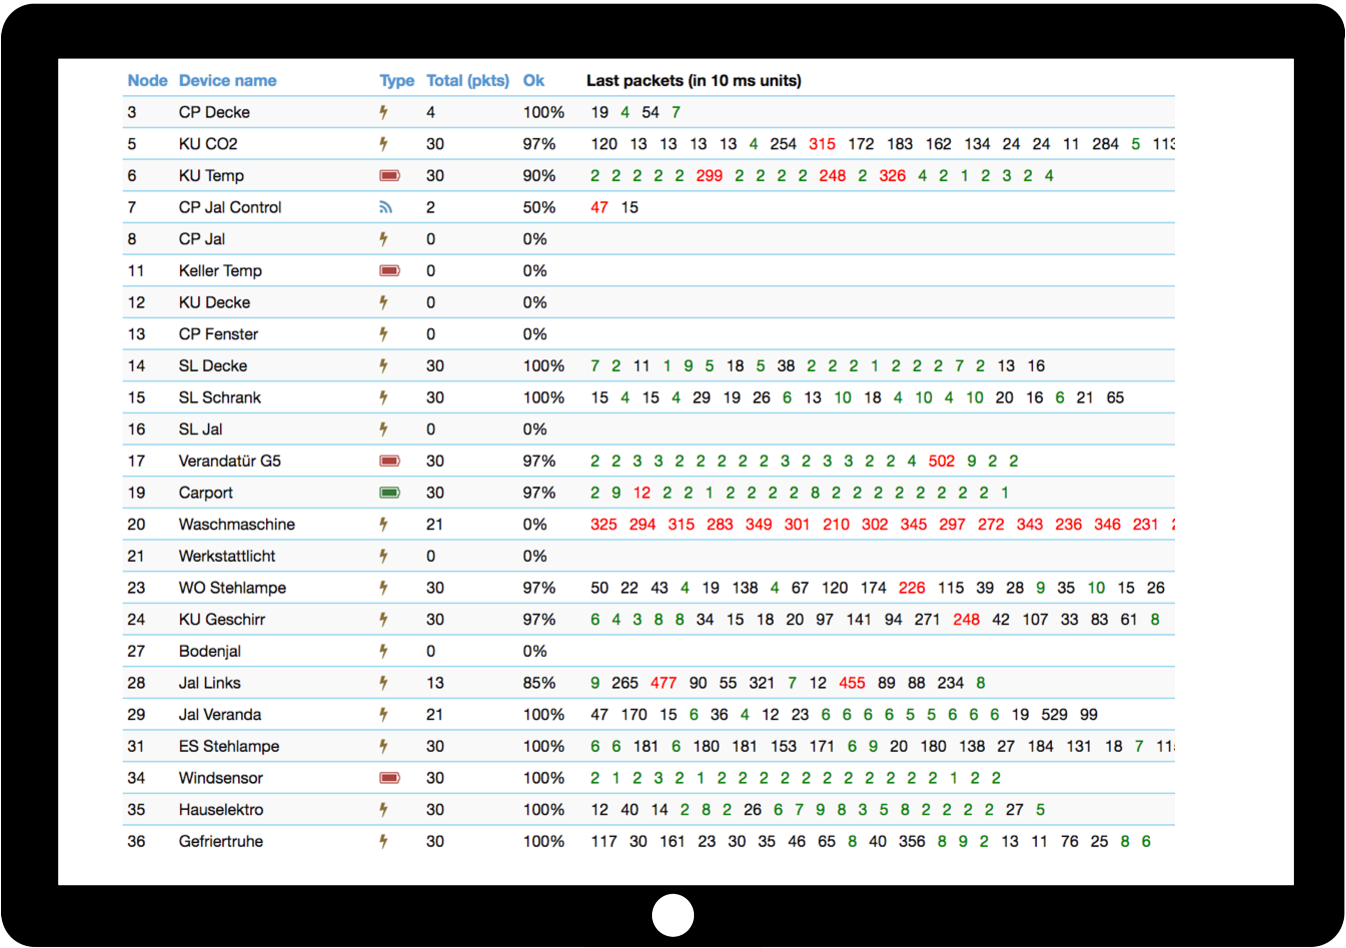
\includegraphics[width=0.7\textwidth]{pngs/cap8/c5timinginfo2.pdf}
\caption{Paket timing of an aged \zwave network}
\label{c5:snifferaged}
\end{center}
\end{figure}

Figure \ref{c5:snifferaged} shows a network that is a bit more complex, has more 
communication and is aged. Again node 20 is a defect device that just needs to be 
replaced. The following interesting patterns can be seen:

\begin{itemize}
\item Node 5 can be reached via routes only but one time not even this worked. There was 
some error. It is possible that the failure of node 20 caused his and then the system 
found an alternative route.
\item Node 6 seems to be in direct range with very stable communication but from time 
to time there is a failed communication. Since this is a battery-operated node, it is 
highly likely that the last communication with the device reaches this device while already 
in deep sleep state. This does not harm the communication at all but is worth monitoring.
\item Node 15 switches between direct communication and routed communication. It seems 
to be right on the edge of having a stable direct link but sometimes - may be when doors 
are open/closed - the direct range does not work anymore.


Anyway, the controller seems to understand that direct range is the by far best option and 
constantly tries to reach the node in direct range. The same pattern can be seen for nodes 29 and 31.
\item Node 24 has an interesting history. For some time, there was a stable direct range 
communication but then it got worse and worse to a point where communication even failed. 
However, the link recovered and the very last communication was again direct, but with a 
slight delay of 80 ms.
\end{itemize}

\section{Network Layer - Weak or Wrong Routes}

It is the best already knowing the troublemaking devices. In this case the status of device 
can be checked quickly and it is possible to dig deeper into the routing layer. 
Figure \ref{c5:neighbortable} shows the routing table of a controller. Technically 
this is not a routing table but a matrix indicating the wireless neighborhoods of devices.
Nevertheless, this a good starting point to investigate deeper. Having many neighbors 
is a good thing since the routing algorithm has many options in case something goes 
wrong. On the other hand, just having one other route to communicate to the rest of 
the network may cause trouble if this route is faulty or moved.

\begin{figure}
\begin{center}
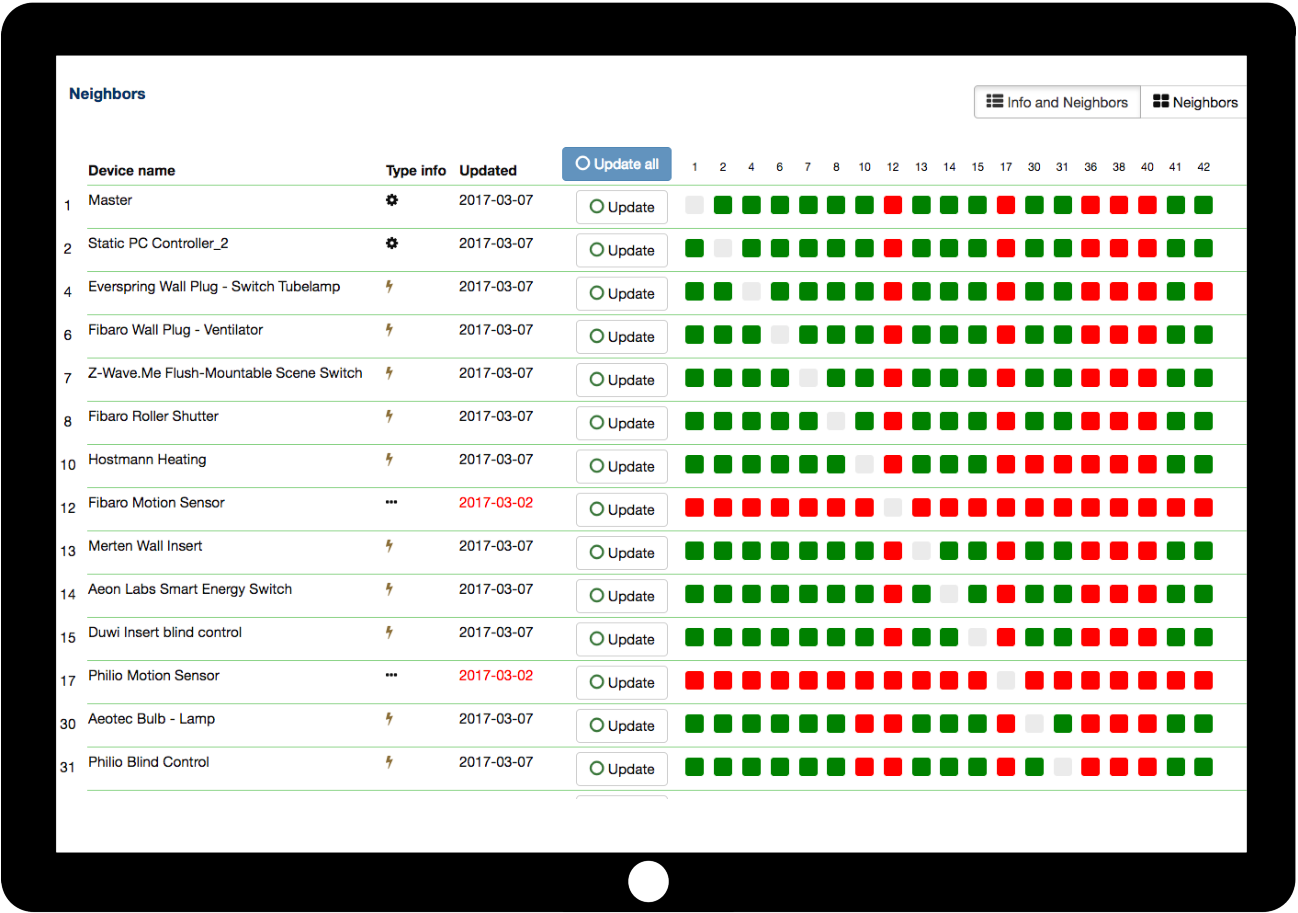
\includegraphics[width=0.7\textwidth]{pngs/cap8/c3neighbortable.pdf}
\caption{Neighbor-Table of a controller}
\label{c5:neighbortable}
\end{center}
\end{figure}

The next step is to check individual routes. The configuration page of every device offers 
a link health check that allows testing the links from this very device to its neighbors.

While the neighborhood table shows if two devices are neighbors, the link test checks how
 good this wireless links is. Unfortunately, not all but an increasing number of devices 
 on the market support this link test. Figure \ref{c5:linktest} shows this dialog 
 within \zweui. Every link has a color indicator (green = ok, 
 red = bad, grey = unknown) and a time stamp that shows when this test was done the 
 last time.

\begin{figure}
\begin{center}
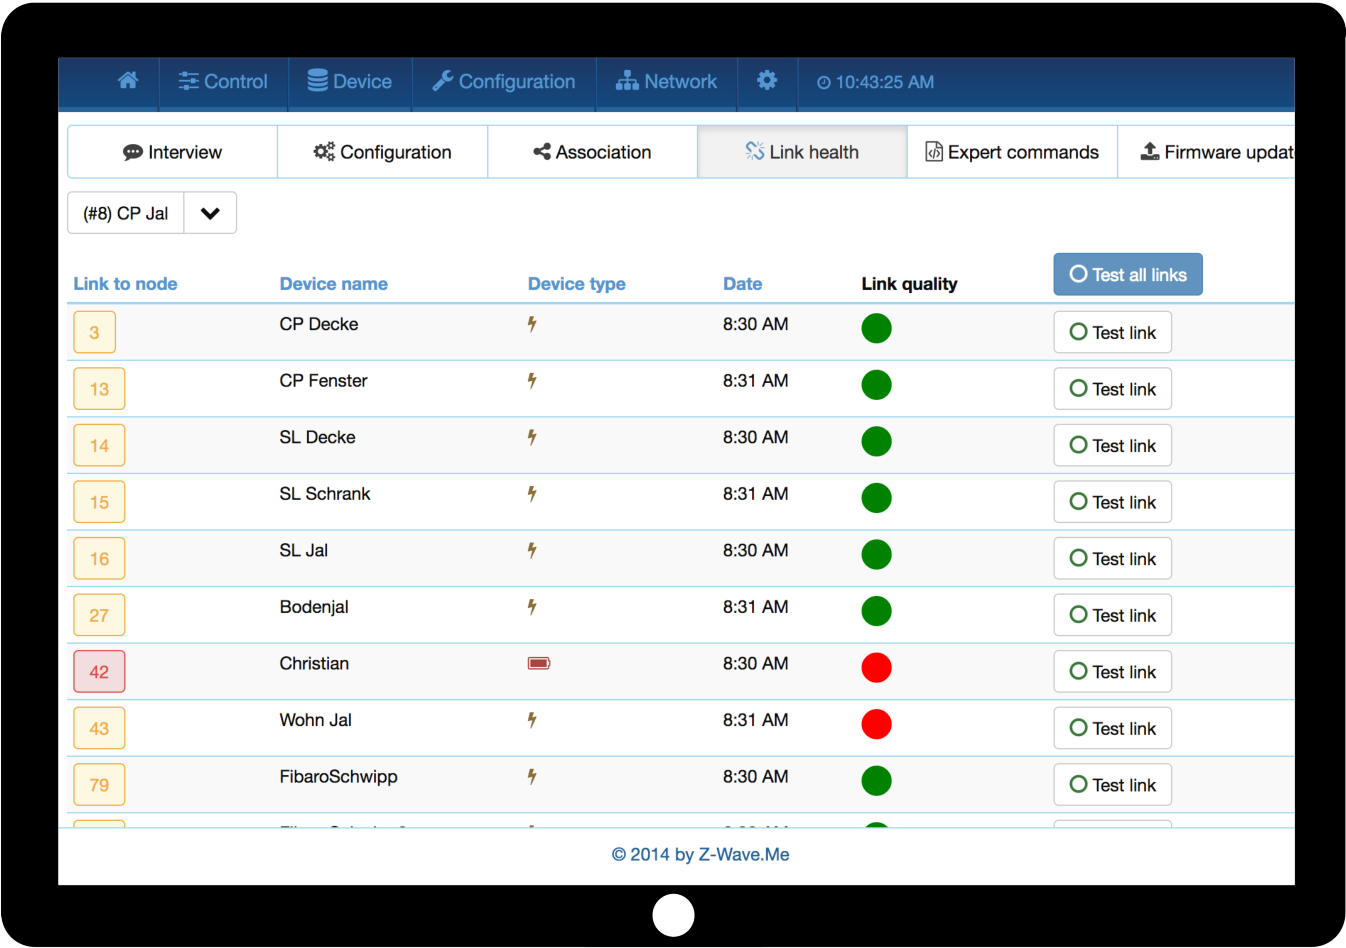
\includegraphics[width=0.7\textwidth]{pngs/cap8/c5linktest.pdf}
\caption{Link test of a node}
\label{c5:linktest}
\end{center}
\end{figure}

Please note that the link check is a momentary analysis only and does not give any 
information about the history of the link quality.


\section{Application Layer Settings}

In the application layer, there is usually no malfunction of a device but wrong 
configurations. \zweui allows changing and monitoring the values.

\subsection{Polling}

Heavy polling of devices causes network traffic leading to delays. A simple look on the 
sniffer as shown in Figure \ref{c5:snifferpak} reveal if there is too much polling.

\subsection{Dead Associations}
\label{c5:deadassoc}

\begin{figure}
\begin{center}
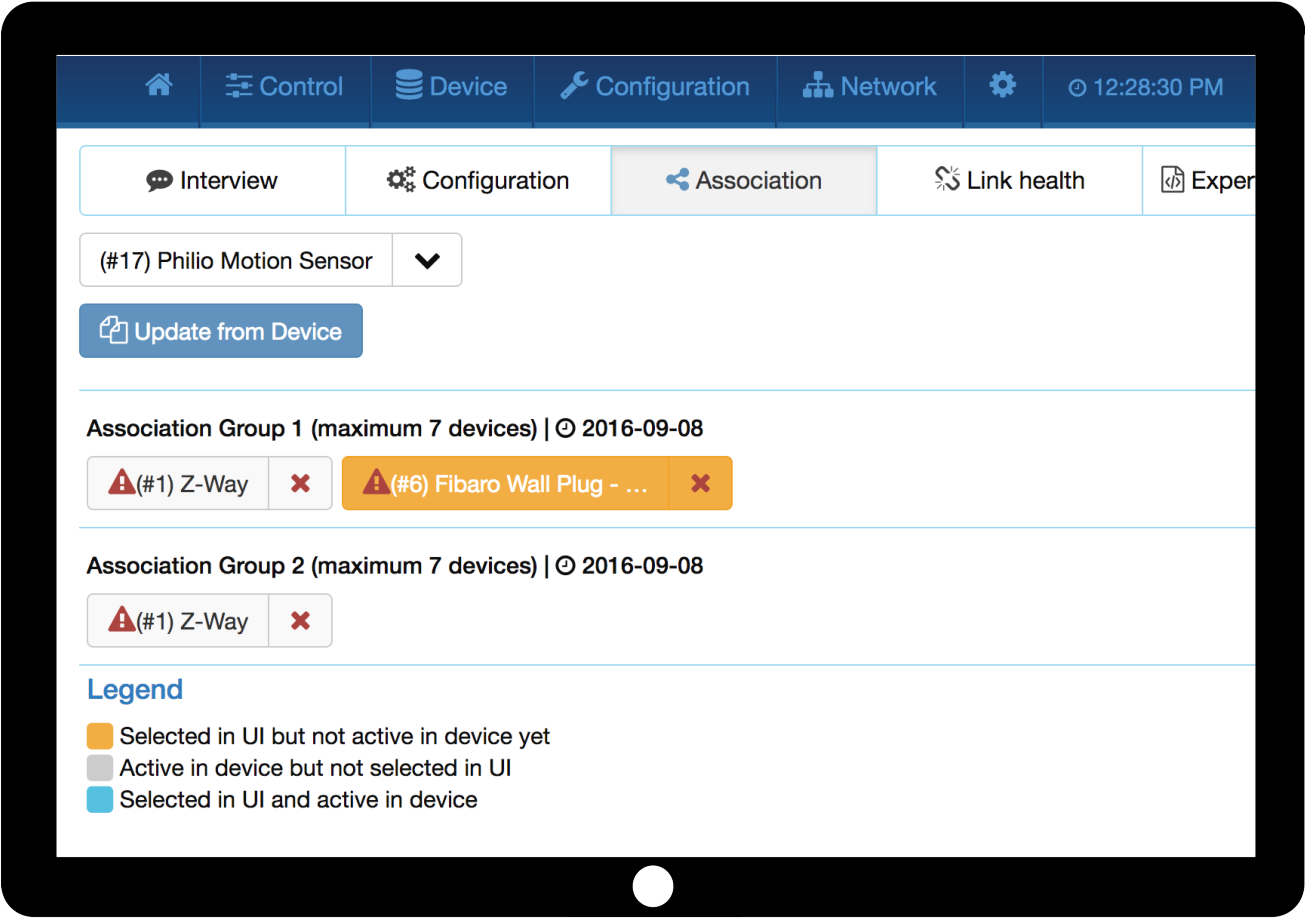
\includegraphics[width=0.7\textwidth]{pngs/cap8/c4association.pdf}
\caption{Association Dialog in \zweui}
\label{c5:assoc}
\end{center}
\end{figure}

Association enable direct communication between devices. In case there are more than one 
device in an association group, they will receive a command one after each other.
A very common problem is that associations are set during the built-up of the network and 
later certain devices are removed or simply fail. If this disappeared node is still 
in an association group, the device will always try to communicate to this node first 
before communicating to other nodes. The result is a delay. The device-specific 
configuration overview as shown in Figure \ref{c5:assoc} displays all association that 
are set. It is possible to recall the current associations from the device and to 
remove or set associations.

\subsection{Wrong Wakeup Settings}

Wrong wakeup settings may either result in too much traffic draining the battery, or in 
too slow response to sensor update requests or configuration changes. The status overview 
page as shown in Figure \ref{c5:citstatus} gives a simple overview of the wakeup settings 
of the different battery-operated sleeping devices. The device-specific configuration settings 
allow changing these settings. Besides the wakeup interval, the setting also allows 
setting/changing the Node ID of the controller holding the mailbox of this device. 
This setting must reflect the correct situation in the network.


\section{Summary}

Table \ref{c5:citsummary} summarizes the possible {\em ``10 root causes of \zwave network problems’’} 
and suggestions how to fix them.

\begin{table}
\begin{tabular}{|p{0.1\textwidth}|p{0.25\textwidth}|p{0.25\textwidth}|p{0.25\textwidth}|}
\hline
No.	&Cause	& How to find ?&	How to fix ?\\
\hline
1	&Noise by other transmitters	&Background Noise Chart	&Find them and turn them off\\
\hline
2	&Noise by other \zwave networks	&Background Noise Chart, Network Statistics	&Talk to the neighbor ;-)\\
\hline
3	&Faulty devices					&Status Page, Failed Node	&Remove them or replace them.\\
\hline
4	&Crazy Devices (always sending)	&Sniffer	&Remove them or replace them\\
\hline
5	&Weak Link						&Neighbor-Table, Link Health in Configuration Page	&Add more routing nodes, move devices\\
\hline
6	&Heavy Fading 					&Timing Infos&Network Reorganization, more devices\\
\hline
7	&Wrong Routing					&Timing Infos &Network Reorganization \\
\hline
8	&Wrong Polling					&Sniffer	&Change and Save \\
\hline
9	&Wrong Wakeup Intervals			&Status Page	&Change and Save \\
\hline
10	&Dead Nodes in Assoc. Groups	&Association display in Configuration Page	&Change and Save \\
\hline
\end{tabular}
\caption{Troubleshooting on \zwave networks}
\label{c5:citsummary}
\end{table}	

